\documentclass[12pt,letterpaper,openany]{article}
\title{Converting PUA characters to Unicode}
\author{Peter S. Baker}
\date{\today}

\usepackage{junicodevf}
\setsansfont{Noto Sans}[Scale=MatchLowercase,Numbers=Lowercase]

\usepackage[hypertexnames=true, plainpages=false, pdfpagelabels]{hyperref}
\hypersetup{pdftex, colorlinks=true, linkcolor=blue, citecolor=blue, filecolor=blue,%
  urlcolor=blue, pdftitle=, pdfauthor=, pdfsubject=, pdfkeywords=,}

\usepackage{graphicx}
\usepackage[table,dvipsnames]{xcolor}

\definecolor{GGOrange}{RGB}{240,74,6}
\definecolor{BrickRed}{RGB}{146,18,6}
\newcommand\textSourceText[1]{{\color{GGOrange}\textsf{#1}}}
\newcommand\textex[1]{\textrm{\textbf{\color{BrickRed}#1}}}
\newcommand{\unic}[1]{{\jSmCond\addfontfeature{Numbers={Uppercase,Monospaced}}#1}}

\begin{document}

\maketitle

\section{The scripts}

Modern best practice, when typesetting documents or creating web pages, is to
avoid the use of characters from the Unicode Private Use Area (PUA) whenever
possible.\footnote{For an explanation, see the \textit{Junicode Manual}, §\,4.1} 
The Medieval Unicode Font Initiative (MUFI) defines more than 
850 PUA characters, and Junicode includes all of them. Junicode also offers alternatives
to all but a handful of these PUA characters, based on standard (non-PUA)
Unicode with OpenType features applied.

OpenType is a powerful technology, but it is undeniably more difficult 
to work with than MUFI’s PUA characters and entities. To copy any character (or its 
corresponding entity) from the MUFI website and paste it into your text is a 
straightforward procedure. By contrast,
to work with OpenType one must locate the correct base character and the 
best OpenType feature, and then figure out how to include the needed markup, 
the syntax of which differs from one application to another.

For many users, a better procedure than struggling with OpenType tags may be to 
enter a PUA code or (better) an entity and let software handle the task 
of marking up the text appropriately. To help with this, the Junicode package
includes a database that maps the relationships between MUFI’s PUA
characters and Junicode’s OpenType features and a script that uses
this database to convert any text’s PUA characters to standard Unicode with
OpenType. This script, \textSourceText{pua2ot}, comes in several flavors, 
all based on the script’s base file, \textSourceText{pua2ot-common.js}:
one is a web app, the second a script to embed in a web page, and a third
a Node module. \textSourceText{pua2ot} works with html/css markup because it 
can easily be edited and can be imported into many applications.

Before you do anything else with \textSourceText{pua2ot}, copy the two font files
\textSourceText{JunicodeVF-Roman.woff2} and \textSourceText{JunicodeVF-Italic.woff2}
into the \textSourceText{pua2ot/fonts} directory in the unzipped
Junicode file tree.

\subsection{With Graphical User Interface}

To use \textSourceText{pua2ot} with a GUI, find the file \textSourceText{pua2ot-gui.html} in
the \textSourceText{pua2ot/gui} directory and double-click or
drag it into an up-to-date web browser. The program will look like this:

\begin{figure}[h!]
  \centering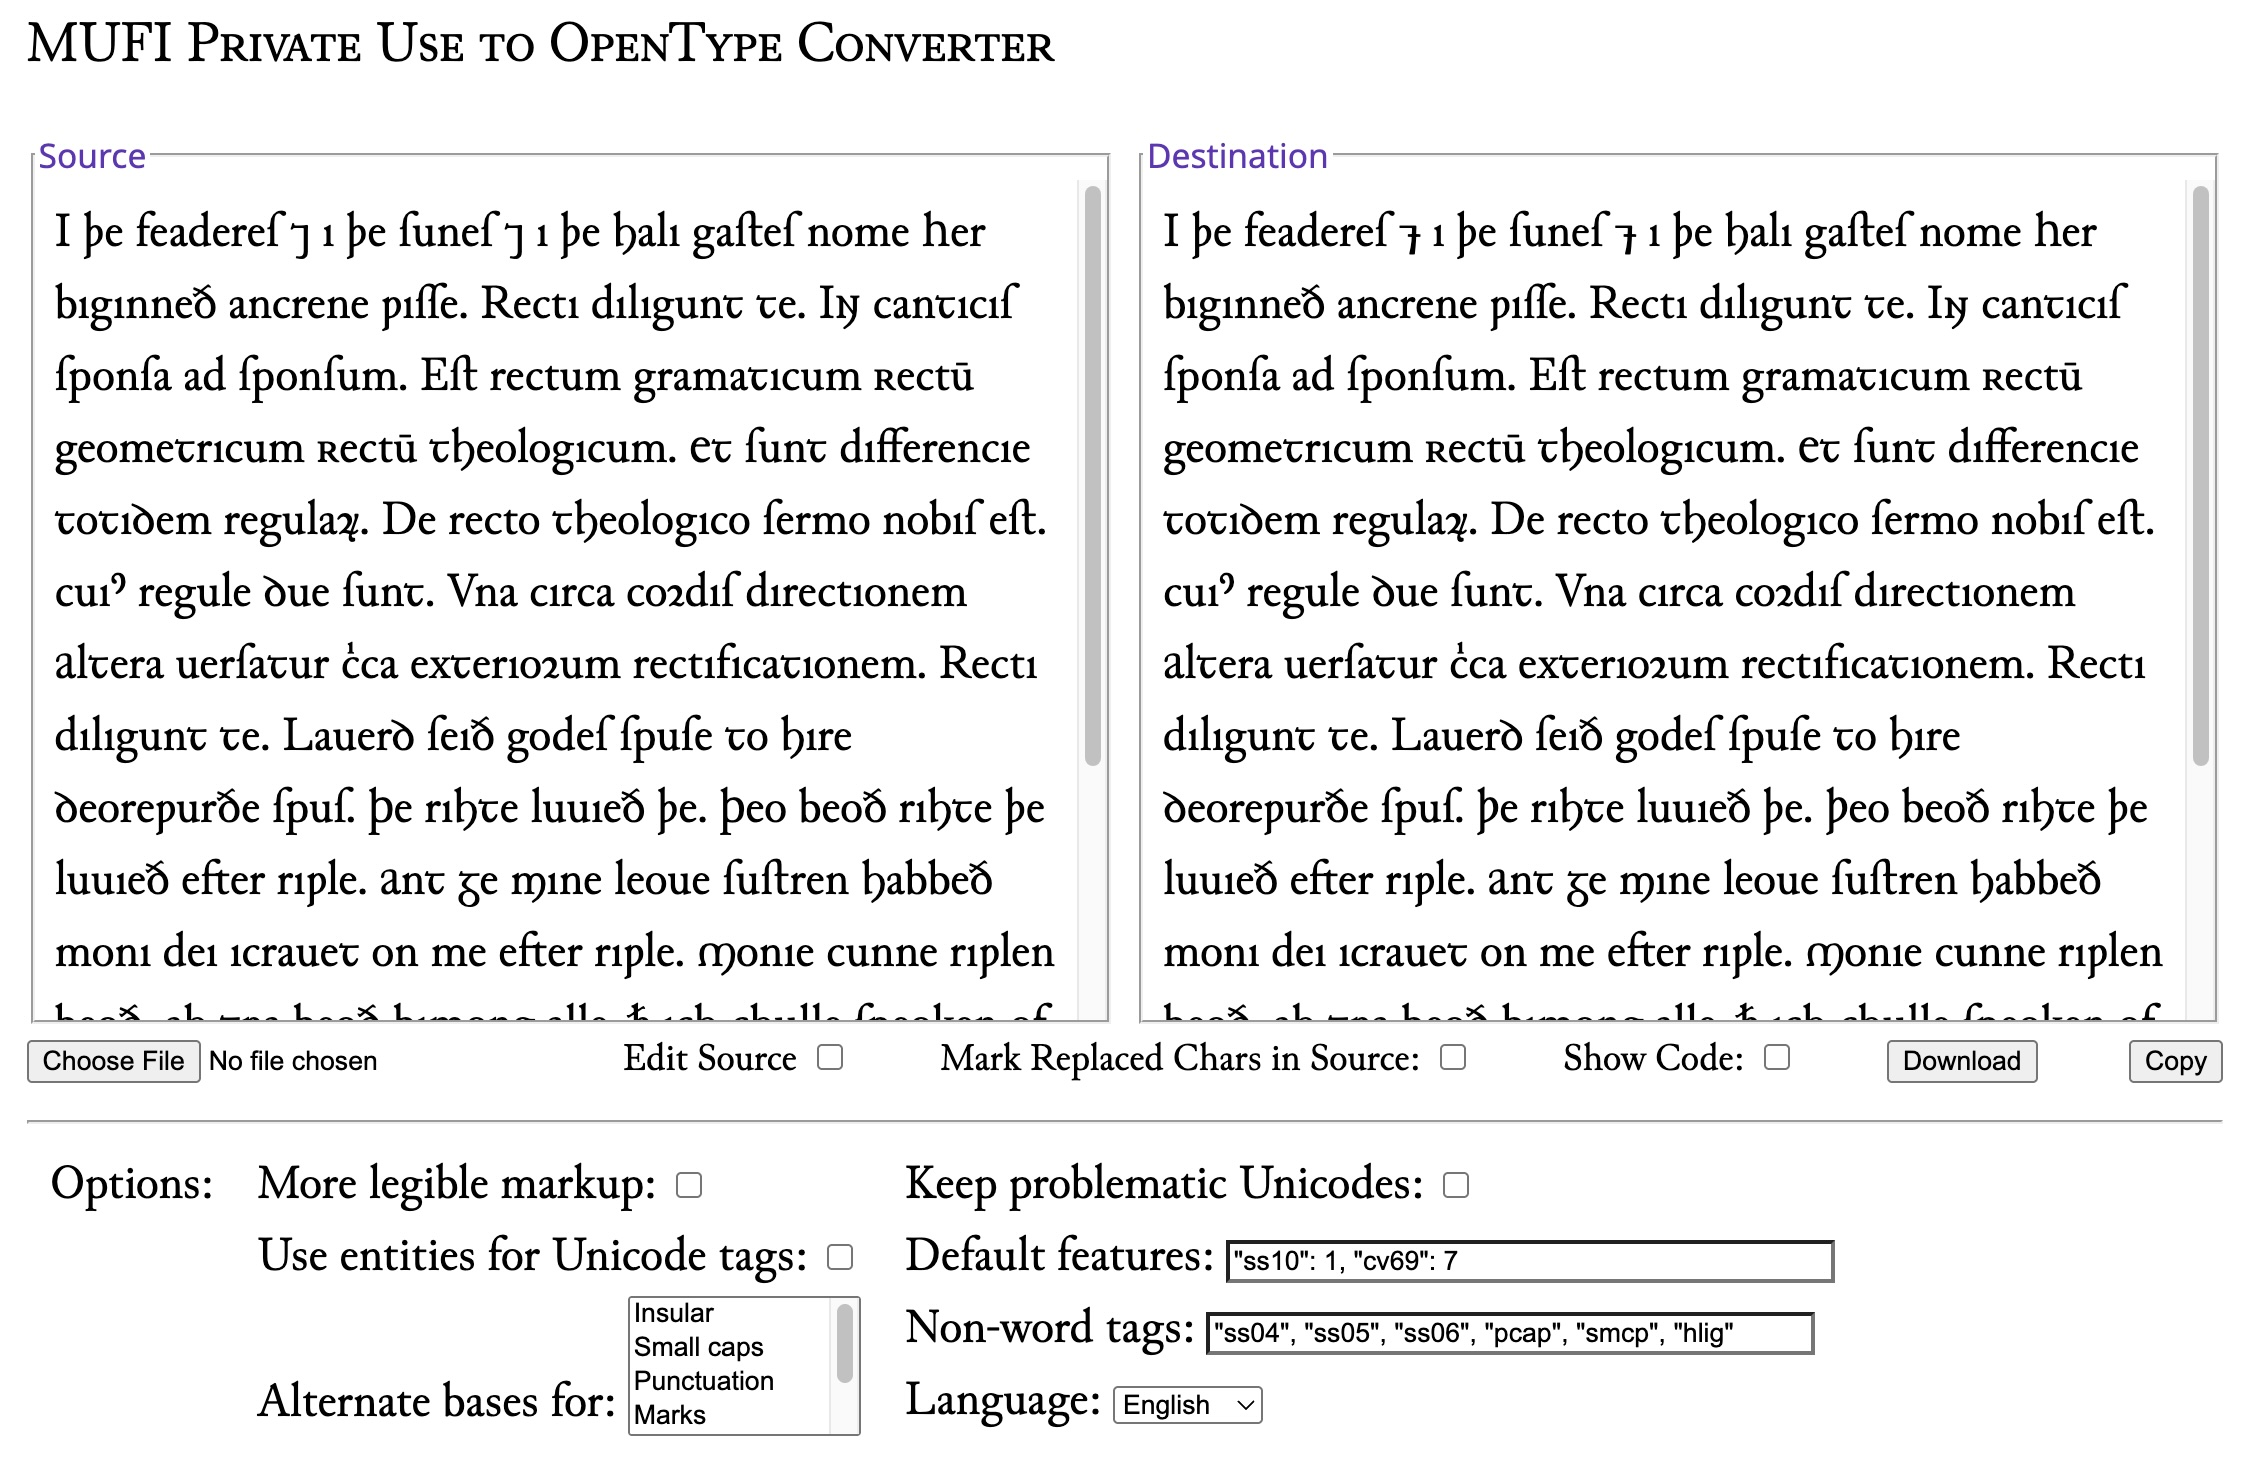
\includegraphics[width=\textwidth]{pua2ot.jpg}
\end{figure}

\noindent The large text-box on the left (initially displaying an excerpt from the 
Middle English \textit{Ancrene Wisse}) is the \textbf{Source Box}; it shows the 
text with PUA characters or entities. The text-box 
on the right is the \textbf{Destination Box}: it displays the result of the 
conversion. These two boxes should look the same: this sameness assures you that 
the conversion has gone well.

Immediately below the text boxes are options that affect their operation. 
To load a text or html file, click the “Choose File” button (“Browse” in some 
browsers) or drag the file into the 
Source Box. To edit the text, check the “Edit Source” box: you can type or 
paste in text when editing is enabled. To see which
characters in the source are being replaced, check the “Mark Replaced Chars in 
Source” box. To view the code that underlies the text displayed in the
Destination Box, check the “Show Code” box. To export the converted text,
click the “Download” or the “Copy” button.

The other options on the page affect the conversion. These are explained below,
in the “Options” section.

\subsection{Embedded in an HTML file}

The second version of the script converts the {\textless}body{\textgreater}
element of any HTML page before it is displayed, with the result that characters 
that could not be searched will become searchable, and the accessibility of the
page will be improved. If the HTML file contains static text, make sure the 
script file, \textSourceText{pua2ot-embed-min.js}, is
in the same folder as your HTML file. Then include 
these lines at the very end of the {\textless}body{\textgreater}:

\begin{scriptsize}\begin{verbatim}<script src="pua2ot-embed-min.js"></script>
<script class="noconv">
    // options.utagEntities = false;
    // options.utagLookup = UTAG_DICT;
    // options.nonWordTags = ["ss04", "ss05", "ss06", "pcap", "smcp", "hlig"];
    // options.keepUnicode = false;
    // options.methodPriority = "compact";
    // options.prefList = ["utag", "zwj", "otag", "entity"];
    // options.defaultTags = {"ss10": 1, "cv69": 7};
    // options.language = "en";
    // options.variantPreferences = [];
    convertAll();
</script>\end{verbatim}\end{scriptsize}

\noindent If your web page loads text dynamically, it won’t work 
simply to include the command \textSourceText{convertAll()} at the end of the 
HTML file, as it will likely be executed before the text is loaded. Instead,
have the process that loads the text trigger an event when the loading is done 
and run \textSourceText{convertAll()} from inside the event handler.

In the html file, include “noconv” in the class list of any element whose
content you don't want converted: the script will skip over such elements.

Other scripts may use this one: simply call the function \textSourceText{convert()},
passing a string as an argument; the function will return a converted string.

In the example above, the commented lines before the \textSourceText{convertAll()} 
command are options, explained in a later section.

\subsection{Node module}

The file \textSourceText{pua2ot-common.js} includes instructions for using it as
a Node module, but if you are not making changes in the programming you can use
\textSourceText{node/pua2ot-node-min.js}, which packages the \textSourceText{pua2ot}
database and program code in a single minified file. The file exports the object
\textSourceText{options} (the options it supplies are listed in the next section)
and two functions: \textSourceText{pua2otNode.cleanup\_string(s)}, which collapses
all sequences of whitespace characters into single spaces, and 
\textSourceText{pua2otNode.convert(text\_buffer, repl\_ent)}, which converts and returns
the text \textSourceText{text\_buffer}, first replacing any MUFI entities if
\textSourceText{repl\_ent} is true.

For an example of how the Node module can be used, consult and run the file 
\textSourceText{test2.js}, especially the \textSourceText{require} statement in 
line 3, the \textSourceText{options} object in line 13, and the invocation of 
\textSourceText{convert()} in line 15.


\section{Options}

In addition to the checkboxes, menus, and text-entry blanks in the web app, the
JavaScript program has an \textSourceText{options} object whose properties can be
manipulated to affect the program's output.

\subsection{More legible markup}

Default: \textSourceText{options.methodPriority="compact"}.
By default, \textSourceText{pua2ot} substitutes standard Unicode characters modified by 
Unicode tag characters (characters from the Unicode tag range) for MUFI PUA characters 
whenever possible. This method produces
relatively compact and accessible web pages. However, Unicode tags are invisible, making 
them hard to edit, and Junicode 
is the only font that uses them in this way: the method is not exactly portable. If 
you check the “More legible markup” box or set
\textSourceText{options.methodPriority="legible"}, \textSourceText{pua2ot} will instead use <span> 
elements with inline style
attributes that turn on OpenType features. The chief advantages of this method are that 
you can see and easily edit the markup, and HTML
elements are more familiar to users than Unicode tags. However, the resulting files
are a good bit bulkier than those that use Unicode tags. You can produce smaller and 
better organized files by running the output of this script through a utility (e.g. the 
\href{https://www.npmjs.com/package/html-style-converter}{Javascript HTML Style 
Converter}) that converts inline styles to a CSS stylesheet.

\subsection{Use entities for Unicode tags}

Default: \textSourceText{options.utagEntities=false}.
If \textSourceText{true}, \textSourceText{pua2ot} uses entities to represent Unicode tags. (These are not 
HTML entities, but unique to Junicode.) This makes the code produced by this script more 
legible, but the entities make the page somewhat larger and can interfere with searching.
It is probably best to use this feature to help you spot problems with your Unicode tags
and turn it off before publishing your text.

\subsection{Keep problematic Unicodes}

Default: \textSourceText{options.keepUnicode=false}. “Problematic Unicodes” 
are characters that are standard Unicode (not PUA) and look like 
variants of common characters, but that many applications do not recognize as 
variants. Examples include dotless i (\textex{ı}, \unic{U+0131}) and the “insular” letter-shapes 
(e.g. \textex{ꝺ}, \unic{U+A77A}). By default, this script replaces these characters with ones that can 
be searched as letters of the alphabet (e.g. \textex{ꝺ} as \textex{d}). To retain the 
“problematic Unicodes,” likely simplifying your markup and making your file smaller, but 
making your text less accessible in some applications, check this box in the GUI version 
or set \textSourceText{options.keepUnicode=true}.

\subsection{Alternate bases}

Default: \textSourceText{options.variantPreferences=[]}.
As a large font with many OpenType features, Junicode often provides more than one way 
to achieve the outcome you want. \textSourceText{Pua2ot} operates by substituting a standard Unicode
\textbf{base} character for a PUA character and then applying OpenType markup to that 
base: \textSourceText{pua2ot} options affect both the base and the markup. This option affects several
classes of character (\textbf{insular} letters, Unicode-encoded \textbf{small caps},
\textbf{punctuation}, combining \textbf{marks}, and \textbf{currency} signs). Select
one or more of the items in this list (use the Shift or Control/Command keys to make
multiple selections) or assign an array to \textSourceText{options.variantPreferences}
to alter the substitutions \textSourceText{pua2ot} makes for many characters in these classes. The
default settings here are chosen to maximize accessibility and minimize the size of 
the output file, but you may have good reasons for preferring alternate choices. For 
example, small caps can by default be searched as their lowercase equivalents (e.g. 
as \textex{a}), but if these small caps make a meaningful distinction in your text,
you may wish readers to be able to search for them by their Unicode values instead 
(\unic{U+1D00} for \textex{ᴀ}). Use this option to maintain that distinction.

\subsection{replaceMUFIEntities}

Default: \textSourceText{options.replaceMUFIEntities=true}.
If \textSourceText{true}, MUFI’s entities (those that
resolve to PUA code points) are replaced by those code points before any other processing
takes place. Set this to \textSourceText{false} if the text you want to convert contains 
no entities and you want to save a little time processing a large text.
Not available in the GUI version, where entities are always converted.

\subsection{Default features}

Default: \textSourceText{options.defaultTags=\{\char"0022ss10\char"0022:\,1,\,\char"0022cv69\char"0022:\,7\}}.
You may wish some OpenType features to be on for the whole document. For example, 
\textSourceText{ss10} “Entities and Tags” must be on in any document that uses Junicode entities or 
Unicode tags. To manage 
your text’s OpenType features, this script needs to know about these default features; 
and when you download or copy your text, they will be recorded in an enclosing <div>. 
Note the format: this is a comma-separated list of key-value pairs, where the keys 
(four-letter tags identifying OpenType features) are in double quotation marks, followed 
by a colon and a number (1 means “on,” but some features (especially the \textSourceText{cvnn} 
“Character Variant” features) require a numerical index).

\subsection{Non-word tags}

Default: \textSourceText{options.nonWordTags=[\char"0022ss04\char"0022,\,\char"0022ss05\char"0022,\,\char"0022%
ss06\char"0022,\,\char"0022pcap\char"0022,\,\char"0022smcp\char"0022,\,\char"0022hlig\char"0022]}.
When “More legible markup” 
is checked, the script applies most <span> tags to whole words, but 
a few to individual characters. This distinction is based on an educated guess as to which OpenType 
features are appropriate to apply to whole words. Sometimes this guess will be wrong. For example, the 
word \textit{rectificaꞇionem} (about halfway through the sample \textit{Ancrene Wisse} text) contains two different 
styles of \textex{t}, but when \textSourceText{cv40} (which transforms default \textex{t} into insular 
\textex{ꞇ}) is applied to the whole word, 
that difference is erased. If you add \textSourceText{cv40} to the list in this box (remember that items in the list 
are enclosed in quotation marks and separated by commas), the feature \textSourceText{cv40} will always be applied to 
single letters rather than whole words. (An alternative to editing this list is to edit the markup 
for this word after you have exported your text.)

\subsection{Language}

Default: \textSourceText{options.language=\char"0022en\char"0022}.
It is important to set the language properly, both here and in your document, since this script
and some of Junicode’s OpenType features behave differently depending on the language. If your 
language is not in the drop-down list (available
only in the GUI version of this script), choose 
“Other” and type in the two-letter code for the language (you can look it up 
\href{https://www.w3schools.com/tags/ref_language_codes.asp}{here}.)

\end{document}